\pdfoutput=1
\documentclass[11pt]{article}

\usepackage[letterpaper,margin=1in]{geometry}
\usepackage[T1]{fontenc}
\usepackage{lmodern}
\usepackage{microtype}
\usepackage{amsmath}
\usepackage{amssymb}
\usepackage{graphicx}
\usepackage{booktabs}
\usepackage{longtable}
\usepackage{siunitx}
\sisetup{range-phrase = { to }, range-units = single}
\usepackage{xcolor}
\usepackage[font=small,labelfont=bf]{caption}
\usepackage[numbers,sort&compress]{natbib}
\usepackage[colorlinks=true,urlcolor=blue,linkcolor=black,citecolor=black]{hyperref}
\allowdisplaybreaks
\setlength{\emergencystretch}{3em}

\hypersetup{%
  pdfauthor   = {Marcus E. Madsen, Audrey K. Christiansen, Jinkwan Han,
                 Jeffrey R. Hill, and Sterling G. Baird},
  pdftitle    = {Experiment-Driven Bayesian Optimization of the Impact Response
                 of Multi-Material 3D-Printed Tensegrity-Inspired Structures},
  pdfkeywords = {Bayesian optimization, tensegrity, multi-material 3D printing,
                 drop testing, design of experiments, data-driven design},
}

\newcommand{\repo}{https://github.com/vertical-cloud-lab/tensegrity-optimization}

\title{Experiment-Driven Bayesian Optimization of the Impact Response of
  Multi-Material 3D-Printed Tensegrity-Inspired Structures}
\author{Marcus E. Madsen\textsuperscript{*}, Audrey K.
  Christiansen\textsuperscript{*}, Jinkwan Han\textsuperscript{*},\\
  Jeffrey R. Hill\textsuperscript{\dag\ddag}, and Sterling G.
  Baird\textsuperscript{\dag\ddag}\\[6pt]
  {\small Department of Mechanical Engineering, Brigham Young University,
  Provo, UT 84602, USA}}
\date{}

\begin{document}
\maketitle

\begingroup
\renewcommand{\thefootnote}{}%
\footnotetext{\textsuperscript{*}M.~E.~Madsen, A.~K.~Christiansen, and
  J.~Han contributed equally. \textsuperscript{\dag}J.~R.~Hill and
  S.~G.~Baird contributed equally. \textsuperscript{\ddag}Corresponding
  authors: \href{mailto:jeff.hill@byu.edu}{jeff.hill@byu.edu} and
  \href{mailto:sterling.baird@byu.edu}{sterling.baird@byu.edu}.}%
\endgroup

\begin{abstract}
Tensegrity-inspired structures of rigid and soft members could cushion
impacts, but their transmitted shock is hard to predict by simulation.
We report a drop-test-driven Bayesian optimization campaign over
three-strut prisms printed in one piece from polylactic acid (PLA) and
thermoplastic polyurethane (TPU). The search space has five geometry
variables, plus infill and filament settings from the third
batch. We scale each candidate to a common mass target before
printing, then 3D print and drop-test it repeatedly. We score
designs by transmissibility (a ratio of filtered top-to-base
peak accelerations) and a mass-weighted rebound index (specimen mass
times the square of a timing-based rebound fraction), both minimized.
Most specimens amplify the peak shock. Across a quasi-random initial batch
and three model-recommended batches (36 specimens), the dominated
hypervolume grew 56 percent. Over a third of that gain comes from the
final batch's best-predicted design, which lowered transmissibility to
0.803, 10 percent below the best initial-batch specimen, and awaits a
re-test. We printed one batch three times to measure repeatability.
Excluding sessions that failed a seating or drift check, which produced
every large deviation, print-to-print scatter in transmissibility was
near 1 percent, so single-print extremes stay provisional. Code and data
are available at \url{\repo}.

\medskip
\noindent\textbf{Keywords:} Bayesian optimization, tensegrity,
multi-material 3D printing, drop testing, design of experiments,
data-driven design
\end{abstract}

\noindent The Supplementary Information is distributed with this preprint
as the ancillary file \texttt{anc/supplementary.pdf}, listed under
``Ancillary files'' on the arXiv abstract page. The text cites its
sections, figures, and tables by S-number.

\section{Introduction}
\label{sec:introduction}

Tensegrity structures are assemblies of rigid compression members
suspended within a continuous network of tension members. Their defining
trait is that no two rigid members contact one another, yielding lightweight assemblies with
high strength-to-weight ratios and tunable nonlinear mechanical
responses~\citep{skelton2009tensegrity, sultan2009tensegrity}. These
properties have made tensegrity attractive from
metamaterial unit cells~\citep{amendola2014experimental,
zhang2018tensegrity, fraternali2015tensegrity} to compliant impact-absorbing
robots developed for planetary landing~\citep{agogino2018superball,
caluwaerts2014superball, sabelhaus2015system, vespignani2018design,
deitrich2022titan}. Recent work has shown that \emph{tensegrity-inspired}
unit cells can be directly 3D-printed and exhibit load-limiting plateaus
under drop-weight impact~\citep{pajunen2019design}. Throughout this paper,
we use \emph{tensegrity-inspired} to refer to printable cells that borrow
the geometry of traditional tensegrity structures without the defining
mechanical conditions of pretensioned members, or cables, associated
with classical tensegrity. In our specimens, the 3D printed cables are
not tensioned as in a true tensegrity structure. Additionally, the
flexible cables share a junction within the vertices of each rigid
strut. Therefore, we do not claim our specimens to be classical
tensegrity structures.

Multi-material fused-deposition modeling (FDM) can be used to pair a
rigid polymer and a soft elastomer within the same part. It has been
used to fabricate energy absorbers which consist of both soft and rigid
portions, including thick-panel origami composites composed of
polylactic acid (PLA) panels and thermoplastic polyurethane (TPU)
hinges~\citep{ye2023multimaterial}, as well as honeycombs of
acrylonitrile butadiene styrene (ABS) interspersed in layers with
TPU~\citep{khatri2024energy}. This rigid-soft multi-material printing
capability makes it possible to fabricate diverse tensegrity-inspired
geometries as well. Although extruded TPU does not behave as an ideal
inextensible cable, its rate-dependent damping is a desirable property
for impact-absorption applications.

Designing such structures capable of energy absorption is a
\emph{Design of Experiments} problem. Strut geometry, cable
cross-section, connectivity (which nodes each member joins), and the
tiling of cells into a lattice span a large configuration space. Each candidate must be physically printed and
tested. Its performance has to be estimated from repeated drops,
because the scatter between drops and between prints can be as large as
the differences between designs. The two relevant impact-performance
metrics (the shock transmitted across the structure and the velocity it
gives back to the protected payload) also partly conflict, so a design
that improves one can worsen the other. Bayesian optimization (BO)
suits this regime. It chooses each next experiment from a probabilistic
model fitted to every result so far, it accounts for measurement noise,
and it can trade off two objectives. BO is widely used to tune
machine-learning models, including
AlphaGo~\citep{chen2018bayesianoptimizationalphago}, and increasingly to
guide physical experiments in materials research, from sustainable
concrete~\citep{ament2023sustainable} to organic laser
emitters~\citep{striethkalthoff2024delocalized}. Closest to this work,
it has been applied to the design of architected
materials~\citep{mo2023accelerated, zhang2021bo}.
The gap this paper addresses is the combination of these two ideas:
multi-material printing of tensegrity-inspired structures, and BO
driven by physical experiments.
Pajunen et~al.~\cite{pajunen2019design} printed tensegrity-inspired
cells under a single fabrication condition with no optimization loop,
and Mo et~al.~\cite{mo2023accelerated} closed a multifidelity BO loop
entirely in simulation. Among the studies reviewed here, prior work
separately demonstrates physical impact testing of printed
tensegrity-inspired structures, rigid-flexible additive fabrication,
and Bayesian optimization of architected materials. We found no prior
report combining these elements in a BO campaign over co-printed
multi-material tensegrity-inspired hardware with physical impact
measurements as the optimization ground truth. In the campaign reported
here, we close the recommend, fabricate, measure, and update cycle three
times (Fig.~\ref{fig:overview}). We trained the surrogate on a seed
batch (batch 1) drawn from a Sobol sequence, and each of three
successive model-recommended batches was fabricated, tested under the
identical protocol, and folded back into the refit that produced the
next.

Our motivating application is protecting the payload of a planetary
lander, where added mass is costly. An absorber there should limit the
peak shock delivered to the payload during touchdown and the motion it
sends back into the payload afterward. These two needs set the two
objectives of this paper. The transmissibility $t_{180}$ compares the
peak acceleration at the top of the structure with the peak at its
base. The mass-weighted rebound index $I_{\mathrm{reb}}$ grows with the
specimen's mass and with a timing-based index of the motion it returns
(Section~\ref{sec:methods:testing}). The mass budget sets a third
condition, that we print every candidate at a common mass. The
printed PLA/TPU three-strut tensegrity prism ($T_3$) studied here is a testbed for developing
and validating the closed-loop workflow. It is not flight hardware, and
it is not the end of the design space we intend to search. Our
contribution is the loop itself, a stepping stone toward optimizing
tensegrity-inspired structures generally, independent of the eventual
application scale.

\paragraph*{Contributions} This paper makes the following contributions:
\begin{enumerate}
  \item A parameterized family of multi-material 3D-printable
    tensegrity-inspired unit cells in which TPU takes the place of the
    tension elements of the traditional topology and PLA struts carry
    compression most of the time. The cells are not prestressed, so
    under impact some tendons stretch while others buckle. The TPU
    tendons are anchored \emph{inside} the strut ends, and a
    constant-mass projection scales every candidate to a common
    material budget before printing
    (Section~\ref{sec:methods:parameterization}).
  \item A characterized drop-tower protocol and two per-specimen impact
    objectives, the transmissibility after nominal channel-frequency-class
    (CFC) 180 filtering~\citep{saej211} and the mass-weighted rebound
    index, each estimated from repeated drops and characterized for
    repeatability (Section~\ref{sec:methods:testing}). The optimizer that
    chose batches 2 to 4 used the rebound index's first-power form.
  \item An experiment-driven BO loop (Ax and BoTorch with a fully
    Bayesian sparse axis-aligned subspace surrogate, SAASBO) that ingests
    the drop measurements, carries each specimen's printed mass, and
    recommends each next batch. Over four measured batches
    (36 specimens), every member of the final Pareto front came from a
    model-recommended batch, and the final batch's best-predicted design
    had the lowest transmissibility measured
    (Sections~\ref{sec:methods:bo} and~\ref{sec:results}).
  \item A measured error budget for drop-tower ranking of printed
    specimens. Three prints of one nine-design batch show that
    print-to-print and seating variation exceed the within-session
    scatter, and a broadband seat gauge flags the largest single-print
    errors (Section~\ref{sec:results:batches}).
  \item A simulation-only benchmark in which multi-objective BO reached
    93\% of a best-known reference hypervolume after 45 designs, against
    76.5 to 79.1\% for three space-filling samplers and a compass search at the same budget,
    and finished ahead on all ten seeds (Sections~\ref{sec:methods:sim}
    and~\ref{sec:results:sim}).
\end{enumerate}

The completed evidence in this paper covers only single-cell,
fixed-topology $T_3$-prism-inspired specimens under one \emph{axial}
drop condition. We plan quasi-static testing as an extension for
future work.
Off-axis and combined loading, controlled fatigue and
damage-accumulation testing, multi-cell behavior, and landing-attitude
variability are likewise future work (Section~\ref{sec:discussion}).
We limit the novelty and generality claims above to this restricted
prototype design space.

\begin{figure}[!tbp]
  \centering
  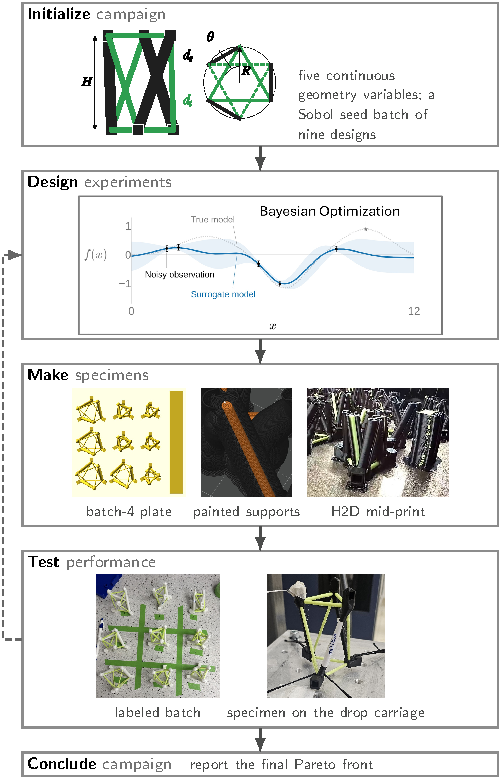
\includegraphics[width=0.52\textwidth]{figures/overview-loop.pdf}
  \caption{Closed-loop, experiment-driven design framework. Initialize and
    Conclude run once, and the dashed arrow returns each tested batch to
    the Design step. \emph{Initialize:} the $T_3$-prism
    design space of Table~\ref{tab:design-vars}
    (Fig.~\ref{fig:design-space}). \emph{Design:} a Gaussian-process
    surrogate fitted to the noisy measurements recommends the next batch
    (Section~\ref{sec:methods:bo}). \emph{Make:} we scale each design to a
    common mass and lay it out as one build plate. We slice the plate with
    PLA supports painted by hand along the TPU tendons and print it in one
    dual-nozzle job, with the hard material (PLA) from the left nozzle and
    the soft material (TPU) from the right
    (Section~\ref{sec:methods:fabrication}). \emph{Test:} we drop-test the
    labeled specimens one at a time on the drop-tower carriage
    (Section~\ref{sec:methods:testing}). \emph{Conclude:} report the
    final Pareto front. The plate render is batch 4, the mid-print frame
    is a later replicate plate, and the labeled specimens are batch 2.}
  \label{fig:overview}
\end{figure}

Section~\ref{sec:background} reviews tensegrity-inspired absorbers,
multi-material printing, and Bayesian optimization.
Section~\ref{sec:methods} introduces the design parameterization,
fabrication, drop-tower protocol and objectives, the BO loop, and the
simulation-only campaign. Section~\ref{sec:results} reports the four
measured batches, the replication findings, the surrogate audits, and
the simulated campaign. Section~\ref{sec:discussion} discusses
implications and limitations, and Section~\ref{sec:conclusions}
concludes the paper.

\section{Background}
\label{sec:background}

\subsection{Tensegrity-Inspired Architectures for Energy Absorption}

Tensegrity prisms and their planar extensions show a softening-stiffening
response under compression~\citep{amendola2014experimental,
zhang2018tensegrity, fraternali2015tensegrity}, which suits impact
mitigation because the structure can absorb input energy at a controlled
force plateau. Santos~\cite{santos2023towardanovel} reported equivalent
viscous damping near 23\% with negligible residual strain per impact in a
tensegrity energy-dissipation metamaterial. Large tensegrity
landers~\citep{agogino2018superball, caluwaerts2014superball,
sabelhaus2015system, vespignani2018design, deitrich2022titan} and
crushable landing systems~\citep{cloutier1966landing,
adams2004merairbag, jackson2014honeycomb} address planetary landing at
much larger scale. Pajunen et~al.~\cite{pajunen2019design} 3D-printed
truncated-tetrahedral tensegrity-inspired unit cells and measured
load-limiting plateaus under drop-weight impact, and Intrigila
et~al.~\cite{intrigila2022fabricationandexperimental} fabricated and
characterized a bistable tensegrity-like unit cell, the closest published
analog to the present cells. Neither study used multi-material FDM or
closed-loop design optimization. Table~S1 of the
Supplementary Information compares the present work with these and
other prior studies.

\subsection{Multi-Material 3D Printing of PLA/TPU Composites}

Rigid-soft multi-material FDM has produced energy absorbers such as
thick-panel origami in which TPU hinges join PLA
panels~\cite{ye2023multimaterial} and ABS/TPU
honeycombs~\cite{khatri2024energy}. Ye et~al.\ encapsulate rigid cores
in continuous soft skins to reduce interface delamination under cyclic
loading, which informed our junction design. Additive manufacturing also
produces tensegrity-inspired architectures with tunable response:
metamaterials that delocalize deformation to resist catastrophic
failure~\cite{bauer2021tensegrity}, lattices whose bandgaps are tuned
by prestrain~\cite{pajunen2021prestrain}, simplex-based
metamaterials~\cite{sabounizawadzka2024experimental}, high-strain-rate
and dynamic characterizations~\cite{almeida2025highstrainrate,
davami2025dynamicanalysis}, and an integrated fabrication-and-validation
workflow for rigid-flexible tensegrity
metamaterials~\cite{wang2026integrated}. None of these studies combines
multi-material FDM with an experiment-driven optimization loop. Layered
PLA/TPU composites~\citep{arifvianto2022mechanicalpropertiesof} bound
the stiffness, strength, and energy absorption of the same material
pair, and FDM PLA fatigue data~\citep{ezeh2018onthefatigue,
vanaei2021multiscaledamageanalysis} inform conservative strut design.
Recent surveys review additively manufactured polymeric energy
absorbers~\citep{bustihan2026recentadvancesin,
liu2026threedimensionalprintedlattice}.

\subsection{Bayesian Optimization for Architected-Material Design}

Bayesian optimization is a sequential, model-based strategy for
optimizing expensive black-box functions with a Gaussian-process (GP)
surrogate~\citep{shahriari2016taking, frazier2018tutorial}.
BoTorch~\citep{balandat2020botorch} and the Ax platform built on
it~\citep{pmlr-v293-olson25a} support batched evaluations and noisy
expected hypervolume improvement (qNEHVI) for multi-objective
problems~\citep{daulton2021nehvi}. Multi-objective BO has also been
developed for engineering design, for example with a weighted Tchebycheff
acquisition~\citep{biswas2022mobotchebycheff}. BO has been applied to
crashworthy multimaterial structures~\citep{liu2019crashworthinessbo},
to additively manufactured lattices under simulated impact
loading~\citep{hertlein2024latticeimpact}, to the equilibrium states of
elastomeric beams for architected beam
networks~\citep{yoo2021elastomericbeams}, to architected-material
design~\citep{mo2023accelerated}, and to additive
manufacturing~\citep{zhang2021bo}. Mo et~al.~\cite{mo2023accelerated}
established a multifidelity BO framework for architected materials that
fuses low-fidelity simulations with high-fidelity ground truth through
nonlinear information-fusion priors~\citep{perdikaris2017nonlinear}. We
shift the emphasis from simulation surrogates to direct experimental
data, which suits materials whose constitutive response is difficult to
calibrate from first principles.

\section{Materials and Methods}
\label{sec:methods}

\subsection{Design Parameterization}
\label{sec:methods:parameterization}

We describe the family of tensegrity-inspired unit cells by four groups
of design variables: the PLA compression members (strut diameter $d_s$),
the TPU tension elements (cable diameter $d_t$), the connectivity
topology (a categorical choice among candidate cells such as
truncated-tetrahedral, prism-based, and octahedral variants), and the
unit-cell tiling (the number of cells $N_x \times N_y \times N_z$ and
their orientation relative to the impact). This paper holds the last
two groups fixed at a single three-strut $T_3$ prism, so every variable
of the present search space is continuous.

\paragraph{Design family and search-space evolution} The reference
instance of this family is a three-strut $T_3$-prism-inspired cell with
circumradius \SI{28.8}{mm} and height \SI{80.8}{mm}. In batches 1 and 2
the search space has five continuous variables
(Table~\ref{tab:design-vars}): the circumradius $R$, the cell height
$H$, the twist angle $\theta$, a single strut diameter $d_s$, and a
single cable (tendon) diameter $d_t$. In a prestressed tensegrity prism,
self-equilibrium fixes the twist between the end
faces~\citep{cao2024tensegrityprism}. Our cells carry no prestress, so
the twist is a free variable. Under the prism's $D_3$ symmetry
all struts are equivalent, and we also give all cables one diameter,
leaving per-orbit (saddle, top, bottom) diameters to a later
extension. From batch 3 the space also
includes two per-specimen sparse-infill densities (strut and tendon),
which the acquisition chooses, and four filament settings (PLA and TPU
nozzle temperature and maximum volumetric speed). A build plate carries
one filament configuration, so we draw these four as one quasi-random
point per batch, and they stay confounded with batch
(Section~\ref{sec:methods:bo}). We fix the joint diameter $d_j$ at
\SI{7.0}{mm} before the projection, so the joint, which sets the
strut-end cage that houses the cable anchors
(Section~\ref{sec:methods:fabrication}), scales with the rest of the cell
(5.4 to \SI{8.1}{mm} as printed in the seed batch) rather than adding a
design variable. Figure~\ref{fig:design-space} shows the variables
on a mid-range prism, six tested specimens at one scale, and an
as-printed specimen.

\paragraph{Constant-mass projection} Cell mass varies severalfold across
the raw design box, so an unconstrained search would partly reward
designs for carrying more material. We therefore scale every candidate
uniformly (all dimensions except the twist) to a common mass target
before printing, converged to within \SI{0.15}{g}. Batches 1 and 2 held
the \emph{solid} CAD mass at $m^{\star} = \SI{30.95}{g}$, the solid mass
of the reference prism. Because PLA struts print at partial infill while
thin TPU cables print near solid, this did not hold printed grams
constant. The tested seed specimens weighed \SIrange{18.50}{22.04}{g}
(coefficient of variation, CV, 5.5\%) and batch~2
\SIrange{17.91}{23.47}{g} (CV 8.7\%), so the surrogate carries each
specimen's weighed mass (Section~\ref{sec:methods:bo}). From batch 3 a
calibrated printed-mass model (Section~S10) let the
projection hold \emph{printed} mass at \SI{20.23}{g}, the mass of the
printed reference specimen. Batches 3 and 4 came in 0.2 to \SI{0.6}{g}
(1 to 3\%) light, with within-batch CVs of 1.7 and 2.3\%. We recorded
two printability screens, a \SI{250}{cm^3} limit on $\pi R^2 H$ and a
\SI{3.0}{mm} minimum printed cable diameter, as warnings and never used
them to reject a design. Nine specimens printed with 2.51 to
\SI{2.78}{mm} cables, including all four batch-4 specimens that reduced
the peak shock. We weigh every specimen to \SI{0.01}{g} but have not
measured printed member dimensions, so the surrogate uses the commanded
post-projection geometry (Section~S2).

\begin{table}[!htbp]
  \centering
  \caption{Design variables of the $T_3$-prism campaign as the BO code
    implements them. Ranges are those of the search space before the
    constant-mass projection, which scales every length of a design.
    The seed batch is a nine-point Sobol draw (fixed seed) over the five
    geometry variables. All specimens print upright on a Bambu Lab~H2D,
    with the prism axis normal to the build plate.}
  \label{tab:design-vars}
  \small
  \begin{tabular}{@{}llccc@{}}
    \toprule
    Variable & Symbol & Range & Units & Active \\
    \midrule
    Circumradius           & $R$       & 25-40 & mm  & batch 1 on \\
    Cell height            & $H$       & 60-110 & mm  & batch 1 on \\
    Twist angle            & $\theta$  & 40-80 & deg & batch 1 on \\
    Strut (PLA) diameter   & $d_s$     & 6.0-12.0 & mm  & batch 1 on \\
    Cable (TPU) diameter   & $d_t$     & 3.0-5.5 & mm  & batch 1 on \\
    Strut infill density   & -        & 12-35 & \%  & batch 3 on \\
    Tendon infill density  & -        & 12-35 & \%  & batch 3 on \\
    PLA nozzle temperature & -        & 212-228 & \si{\celsius} & batch 3 on\textsuperscript{a} \\
    PLA volumetric speed   & -        & 20-30 & \si{mm^3/s} & batch 3 on\textsuperscript{a} \\
    TPU nozzle temperature & -        & 235-245 & \si{\celsius} & batch 3 on\textsuperscript{a} \\
    TPU volumetric speed   & -        & 2.2-3.6 & \si{mm^3/s} & batch 3 on\textsuperscript{a} \\
    Joint diameter (fixed) & $d_j$     & 7.0 & mm  & - \\
    \bottomrule
  \end{tabular}\\[2pt]
  {\footnotesize \textsuperscript{a}One value per print job (a plate
  carries a single filament configuration), so per-batch rather than
  per-specimen.}
\end{table}

\begin{figure*}[!tbp]
  \centering
  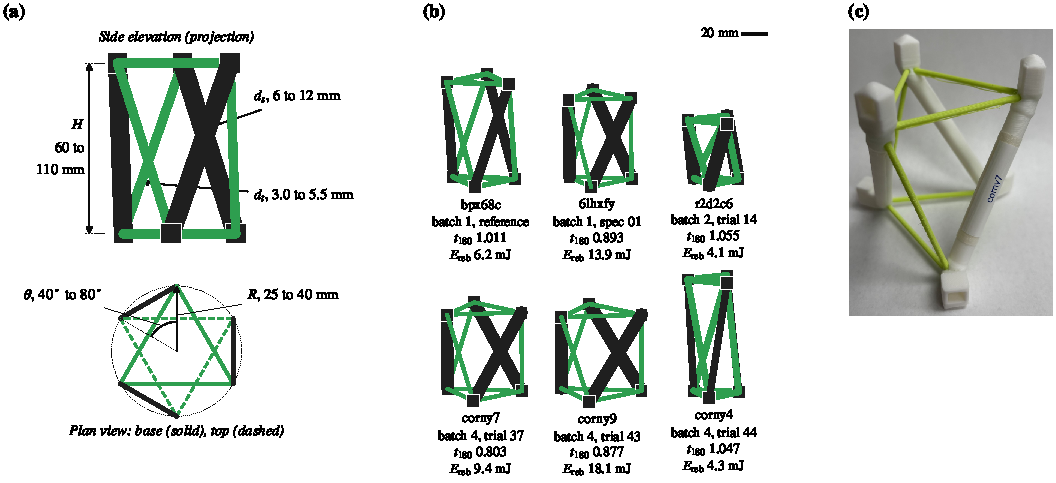
\includegraphics[width=\textwidth]{figures/design-space.pdf}
  \caption{Design space of the $T_3$-prism campaign. \emph{(a)} A mid-range
    design of the five-variable box ($R = \SI{32.5}{mm}$,
    $H = \SI{85}{mm}$, $\theta = 60^\circ$, $d_s = \SI{9}{mm}$,
    $d_t = \SI{4.25}{mm}$, before scaling to the mass target), labeled
    with the bounds of each variable. The side elevation is an
    orthographic projection, so each end triangle appears as a line, and
    $H$ is the vertical distance between the planes through the joint
    centers. The plan view shows the base triangle (solid), the top
    triangle (dashed), the circumradius $R$, and the twist $\theta$
    between them. \emph{(b)} Six tested specimens at their commanded,
    post-projection geometry at one common scale (\SI{20}{mm} bar), labeled with the
    batch, the Ax trial (or the Sobol spec of a seed specimen), and the
    measured $t_{180}$ and $E_{\mathrm{reb}}$. \emph{(c)} Specimen corny7
    as printed, with its ID label around one strut. The drawings show PLA
    struts in black, TPU tendons in green, and the square strut-end
    housings. We printed specimen corny7 in white PLA.}
  \label{fig:design-space}
\end{figure*}%

\subsection{Multi-Material Fabrication}
\label{sec:methods:fabrication}

We printed every specimen in one dual-nozzle job on a Bambu Lab~H2D,
with PLA struts and TPU tension elements, so the build needs no filament
swap (Fig.~\ref{fig:overview}, Make panel). The TPU tendons are anchored
\emph{inside} the ends of each PLA strut. The cables meeting at a strut
end join within a printed cage, a captive TPU core inside a PLA shell
(Design~F of the joint study in Section~S3), and leave it
through discrete outlets. This keeps the soft-rigid interface in
internal pockets rather than at an exposed surface. It inverts the
material roles of the wrapping strategy of Ye
et~al.~\cite{ye2023multimaterial}, in which a soft skin covers a rigid
core, so that work is a precedent for co-printing rather than a
validation of this junction. Because near-vertical tendons are
otherwise unsupported, we disabled automatic support generation and
painted PLA edge supports along each tendon in the slicer
(Section~S4, with a timelapse of a full plate in
Fig.~S2). The most frequent logged defects
are TPU stringing and small bubbles in diagonal tendons, and two seed
specimens lost tendon strands during support removal
(Section~S6). The TPU fed from a heated dry box held
at 7 to \SI{11}{\percent} relative humidity, logged per print. Midway through the
seed batch, a cold pull and a move to a dedicated high-flow
\SI{0.6}{mm} nozzle cleared a partial clog of the TPU extruder, and the
print key flags the affected specimens. Table~S2
lists the print parameters transcribed from the archived slicer
projects (Section~S5).

\subsection{Experimental Characterization}
\label{sec:methods:testing}

We drop-tested every specimen on one instrumented fixture under one
protocol.

\paragraph{Drop-tower fixture} The printed specimen rode upright on the
free-fall carriage plate of a Lansmont Model~23 shock test system, which
we raised \SI{1.524}{m} (\SI{60}{in}) along guide rails and released.
The plate landed on a single \SI{12.7}{mm} (\SI{0.5}{in}) Shore 60~OO polyurethane
cushioning sheet, which shaped the landing into one sharp base pulse of
roughly \SI{1.6}{ms}. We chose this surface in a blinded crossover
experiment over three candidate mat arrangements, and unlike a felt
stack it did not measurably compact over 100-drop sessions. We monitored
rig health through the impact velocity change $\Delta v$ recovered from
the base accelerometer. Over an uninterrupted 100-drop session (one
specimen's consecutive drops in a single seating) its
coefficient of variation was 0.54\% with no drift, and we checked every
campaign session against this baseline (Section~S7).

\paragraph{Instrumentation and signal processing} A single-axis
piezoelectric accelerometer on the carriage plate recorded the base
input and triggered the acquisition, and a triaxial accelerometer
(Dytran 3133A4) seated in a printed pocket at the specimen's top vertex
recorded the transmitted response. We cross-calibrated the two
base-capable channels in place over 15 co-located drops (ratio
$0.953 \pm 0.001$ at matched filtering). We sampled at \SI{1.25}{MHz}
over a \SI{100}{ms} record with a \SI{2}{ms} pre-trigger and low-pass
filtered every channel with a zero-phase two-pole Butterworth filter run
forward and backward at the corner $1.65 \times \mathrm{CFC}$ of each
SAE~J211/1 channel frequency class~\citep{saej211}. Because the corner
is applied to each pass rather than to the combined response, this
passband is about 20\% narrower than the one the standard specifies. On
the drop of Fig.~\ref{fig:transmissibility-trace}, the standard's
filter gives the same $t_{180}$ and a CFC-1000 ratio of 1.287 in place of
1.204. CFC-180 is the reporting class for peak metrics, and
CFC-1000 is a higher-bandwidth diagnostic.
Figure~\ref{fig:transmissibility-trace} shows both channels of one drop
at both filter classes.

\begin{figure}[!tbp]
  \centering
  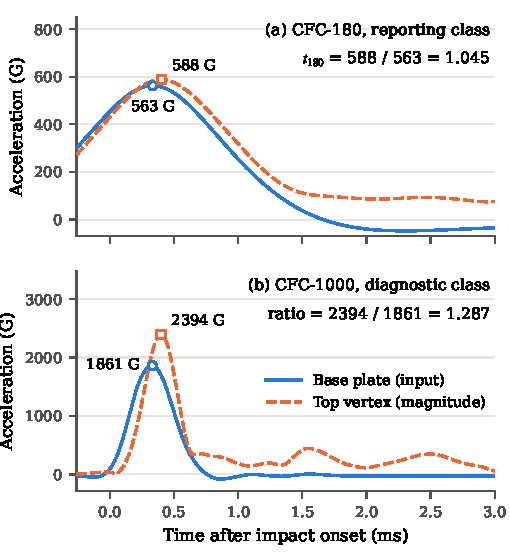
\includegraphics[width=0.55\textwidth]{figures/analysis/transmissibility-trace-57vqhX-drop50.pdf}
  \caption{Base-plate input and top-vertex response for one
    commissioning drop, shown to illustrate the transmissibility
    definition. The specimen is 57vqhx from the pre-campaign
    print-defect study (2026-07-28, event 50 of its session), dropped
    from \SI{1.524}{m} (\SI{60}{in}) onto the earlier stack of four felt pads and one
    cardboard sheet. Campaign drops land on the polyurethane surface
    instead. Both channels are low-pass filtered as SAE~J211/1
    specifies, and the top-vertex trace is the magnitude of the three
    filtered axes. The zero-phase CFC-180 filter spreads the
    sub-millisecond pulse in both directions in time, so its traces
    are already nonzero at impact onset. (a)~At CFC-180, the reporting
    class, the peak ratio
    gives $t_{180} = 1.045$ (peaks of 588 and \SI{563}{G}). (b)~At
    CFC-1000, the diagnostic class, the same drop gives 1.287 (2394 and
    \SI{1861}{G}). The campaign
    pipeline's narrower filter gives 1.045 and 1.204.}
  \label{fig:transmissibility-trace}
\end{figure}

\paragraph{Sessions and objectives} Seed sessions recorded 101 drops per
specimen (103 for autv5r). We discarded the first 2 drops of each
session as seating warm-up, so 99 stabilized drops (101 for autv5r)
enter each seed mean. Truncating the seed sessions to their first 20
stabilized drops left the transmissibility ranking of all nine seed
specimens unchanged (Section~S7), so later sessions
recorded 20 to 22 drops, leaving 18 to 20 stabilized drops per
specimen. Each session yields two objectives, each a stabilized mean
whose standard error enters the surrogate's noise model
(Section~\ref{sec:methods:bo}):
\begin{equation}
  \begin{aligned}
    t_{180} &\;=\; \frac{\max_t\,\lVert \mathbf{a}_{\mathrm{top}}(t)\rVert_{\mathrm{CFC180}}}
                        {\max_t\,\lvert a_{\mathrm{base}}(t)\rvert_{\mathrm{CFC180}}},\\
    e_{\mathrm{reb}} &\;=\; \frac{g\, t_{\mathrm{second}}}{2\,\Delta v},
    \qquad
    I_{\mathrm{reb}} \;=\; m\, e_{\mathrm{reb}}^{2}.
  \end{aligned}
  \label{eq:objectives}
\end{equation}
The \emph{transmissibility} $t_{180}$ is the peak magnitude of the
filtered triaxial top-vertex response over the peak filtered base input
within the impact window. We use the term in the shock-testing sense of
cushioning and packaging drop tests, a ratio of filtered peak
accelerations across the specimen under a single transient, not the
steady-state frequency-response function of vibration isolation. The two
peaks need not be simultaneous, and the filter class is part of the
definition. Values above unity mean the structure amplifies the peak
shock reaching its top vertex.

The second objective is the \emph{mass-weighted rebound index}
$I_{\mathrm{reb}}$, reported in milligrams, and lower is better. It is
built on the rebound fraction $e_{\mathrm{reb}}$, the hop speed of the
top vertex estimated from the time to its second contact,
$t_{\mathrm{second}}$, under a ballistic
assumption~\citep{bernstein1977listening}, divided by the measured base
velocity change $\Delta v$. Weighting by the specimen's weighed mass $m$
keeps grams in the objective, because equal rebound fractions on
specimens of different mass are not equivalent outcomes for a payload.
We adopted $I_{\mathrm{reb}}$ after the final batch. The optimizer that
recommended batches 2 to 4 minimized the first-power form
$E_{\mathrm{reb}} = e_{\mathrm{reb}}\, m\, g\, h$ (in mJ, with $h$ the
drop height) instead, so the predictions it archived are in
$E_{\mathrm{reb}}$. Because $g h$ is the same for every drop,
$E_{\mathrm{reb}}$ ranks designs exactly as $m\,e_{\mathrm{reb}}$ does,
and squaring the rebound fraction reverses the order of only 21 of the
595 pairs of the 35 tested designs, 16 of them within 5\% (Spearman
$\rho = 0.990$ between the two orderings; Section~S8).
Where we quote rebound as a dimensionless descriptor we use the velocity
loss index $\mathrm{VLI} = 1 - e_{\mathrm{reb}}$ (higher is better),
which spans 0.937 to 0.986 across the 54 tested specimens.

\paragraph{What the rebound fraction measures} The rebound fraction is
a timing index, not a coefficient of restitution. We tracked the
instrumented top vertex in high-speed video (\SI{959}{fps}, three drops
per specimen) for the 27 specimens of batch 4 and the first two prints
of batch 3 (Section~S8). After impact the vertex rises
12.5 to \SI{28.4}{mm} back toward its resting height rather than
leaving in free flight, where the ballistic reading implies a hop of
only 0.3 to \SI{5.9}{mm}. The video's ratio of rebound to arrival speed
is about four times the ballistic estimate (the ballistic value is a median 0.24 of the video ratio), and the
two rank the specimens similarly but loosely (Spearman $\rho = 0.52$,
$p = 0.005$). The measured $\Delta v$ also includes the carriage's
bounce off the mat (0.56 to \SI{0.64}{m/s} in seven filmed drops),
which inflates it by about the same factor for every design. We
therefore use $e_{\mathrm{reb}}$ only to rank designs, and
$I_{\mathrm{reb}}$ is a ranking score that penalizes designs, and grams,
that send more motion back to the payload, not a measured
energy. The pipeline searches for the second contact between 15 and
\SI{70}{ms} after impact (Table~S5). Three of the
35 first-print sessions have a mean $t_{\mathrm{second}}$ within
\SI{0.7}{ms} of the start of that window (r2d2c6, drran3, and corny4,
which hold the three lowest $I_{\mathrm{reb}}$ values, 3.9 to
\SI{4.1}{mg}), and one sits within \SI{0.9}{ms} of its end (drran1).
For these four sessions the rebound fraction is bounded by the search
window rather than measured.

\paragraph{Session diagnostics and replication} The within-session
per-drop CV of $t_{180}$ spans 0.06 to 2.0\% across all 54 tested
specimens (0.17 to 0.48\% in the seed batch). These values describe
repeated drops of one specimen in one seating, not print-to-print or
seating-to-seating repeatability, and serial dependence among drops may
make $s/\sqrt{n_{\mathrm{drops}}}$ optimistic. As an advisory check on
seating, we computed a \emph{seat gauge} for every session, the ratio of
its CFC-1000 to its CFC-180 transmissibility. CFC-1000 keeps short,
sharp spikes, such as a loosely seated specimen or top sensor knocking
against its seat, that CFC-180 smooths out. The gauge read 1.00 to 1.07
on most sessions, and we call a session whose gauge reaches 1.145 (1.15
to two decimals) a \emph{re-seat candidate}, to be re-mounted and
re-tested before its value drives a decision. The seed attenuator read
within 0.14\% of its campaign value in a shorter seating on the
previous day. Three prints of the
batch-3 designs put the standard deviation between specimens and
seatings at 0.0087 in $t_{180}$ once sessions that fail the gauge or
carry a drift flag (a stabilized $t_{180}$ trend steeper than 0.06\% per
drop with $p < 0.01$, or a change of more than 2.5\% between the first
and last five stabilized drops; Section~S7) are set aside,
and the two largest deviations, 10
and 20\% above their design medians, both failed the gauge
(Section~\ref{sec:results:batches}). We therefore adopted a
between-seat replication rule: a single-seating value that would drive a
decision (a batch extreme, a claimed attenuator, a front membership)
needs confirmation on an independent re-seat before we treat it as a
design property. The specimens stay elastic in these drops, so
crush-energy metrics such as specific energy absorption are not
recoverable from them; a planned quasi-static campaign will supply them
(Section~S9).

\subsection{Experiment-Driven Bayesian Optimization Loop}
\label{sec:methods:bo}

The loop maintains a Gaussian-process surrogate over the design space of
Section~\ref{sec:methods:parameterization}. After each round of
experiments we refit it and maximize an acquisition function to
recommend the next batch. We pose the campaign as a two-objective
minimization of the transmissibility $t_{180}$, which bounds the peak
shock the payload feels during impact, and the mass-weighted rebound
index $I_{\mathrm{reb}}$, which penalizes the motion thrown back into it
afterward (Eq.~\eqref{eq:objectives}). The optimizer recommended batches
2 to 4 under the first-power form $E_{\mathrm{reb}}$, any later batch
minimizes $I_{\mathrm{reb}}$, and every measured specimen has both
values, so later results stay comparable with the existing front. We
implement the loop in Ax~\citep{pmlr-v293-olson25a} over
BoTorch~\citep{balandat2020botorch}, with noisy expected hypervolume
improvement (qNEHVI)~\citep{daulton2021nehvi} as the acquisition. The
search space is fully continuous, including the process variables added
in batch 3, so it needs no categorical encoding.

\paragraph{Surrogate and noise model} The surrogate is the fully
Bayesian sparse axis-aligned subspace model
(SAASBO)~\citep{eriksson2021saasbo}, a Mat\'ern-5/2 kernel with automatic
relevance determination whose length scales carry sparsity-inducing
priors and are marginalized by Markov-chain Monte Carlo with the
No-U-Turn Sampler (NUTS) rather than point-estimated. Every fit that
generated a batch, and every archived prediction, used the BoTorch
default budget of 512 warmup steps and 256 samples, thinned to 16
retained draws (Ax~0.4 for the early rounds and Ax~0.5.0 from the
batch-3 refit). We prespecified SAASBO because marginalizing the
hyperparameters tends to improve uncertainty quantification at the small
sample sizes of physical campaigns, and we make no claim that it
outperforms a point-estimated GP here (Section~\ref{sec:results:audits}).
Inputs are normalized to the unit cube and outputs standardized. We
supply each observation's noise as a fixed variance. For $t_{180}$ it is
the squared standard error of the stabilized mean,
$\sigma_t^2 = s_{\mathrm{drop}}^2 / n_{\mathrm{drops}}$. For
$I_{\mathrm{reb}}$ it adds two relative errors in quadrature,
$(\sigma_I/I_{\mathrm{reb}})^2 = (2\sigma_e/e_{\mathrm{reb}})^2 +
(\sigma_m/m)^2$, where $\sigma_e$ is the standard error of the session's
mean rebound fraction and $\sigma_m = \SI{0.457}{g}$, the standard
deviation of printed mass over three prints of one seed design (spec 08),
stands in for print-to-print variation at a fixed design. The refits
through batch 4 used the same construction for $E_{\mathrm{reb}}$,
without the factor of 2. This noise model estimates the response of the
tested specimen in its seating, not of a fresh print of the same design.
We ingested the nine second-print specimens of batch 3 as distinct
completed trials at identical coordinates, each with its own weighed mass
and standard error, so later refits observe design-level replicates.
Batch-sampling schemes can make the choice between replicating an
observed design and sampling a new one under heteroscedastic
noise~\citep{vanbeek2021batchnoise}; in this campaign a fixed replication
rule made it.
Because the variances are supplied as known, no inferred noise term
absorbs replicate disagreement and the fit must explain it through the
inputs. Section~\ref{sec:results:audits} shows what that cost in
held-out skill. The third print of batch 3 was tested after the last
refit reported here and has not entered the fit.

\paragraph{Mass treatment} The constant-solid-mass projection of batches
1 and 2 left printed mass correlated with the shape variables and with
$t_{180}$ in the seed batch (Section~\ref{sec:results:seed}), so we keep
mass explicit. $I_{\mathrm{reb}}$ uses each specimen's weighed mass, and
$t_{180}$ stays a ratio because payload peak acceleration is a damage
criterion that does not scale with specimen mass. The fit that chose
batch~2 took the five geometry coordinates as inputs and modeled printed
mass as a separate tracking metric. From the refit that chose batch 3,
each specimen's weighed mass is also an input of the objective
surrogates, and candidate generation holds it at the mass target.
Batches 3 and 4 then held \emph{printed} grams constant, and across all
53 specimens with a weighed mass, printed mass explains about 1\% of the variance in
transmissibility ($r = 0.12$).

\paragraph{Budget and seeding} We drew the nine seed designs as the
first points of a scrambled Sobol sequence~\citep{sobol1967distribution,
owen1998scrambling}, the initialization step of Ax, with a recorded seed
(0), and printed them with the fixed reference prism (S0). A Sobol
sequence covers the design box more evenly than the same number of
independent random draws. Optimization then proceeds in batches of
$q = 9$ prints, one build plate per batch. We report three
model-recommended batches (Ax trials 10 to 18, 28 to 36, and 37 to 45);
the numbering gap is a draft batch we regenerated before printing when
we simplified the batch-level filament handling. From batch 3 the four
filament settings take one quasi-random point per batch, so they are
confounded with batch and we report them as unidentified. We archive
the random seeds, the full experiment state, and the recommendation
tables of every round with the campaign code (Data Availability
Statement).

\subsection{Simulation-Only Campaign}
\label{sec:methods:sim}

To test the optimizer on a problem whose front we can map, we
also ran a campaign entirely in simulation. The simulator is a
MuJoCo~\citep{todorov2012mujoco} model of the drop tower with rigid
PLA struts, tension-only TPU tendons, and an impact-surface contact
calibrated once against the reference prism (S0). It reports $t_{180}$
after the CFC-180 filter as SAE~J211/1 specifies, rather than the
narrower bench variant of Section~\ref{sec:methods:testing}. We fix
printed mass at \SI{20.23}{g},
and the search varies four shape ratios, with printed tendon diameter
of at least \SI{3.0}{mm} and envelope volume $\pi R^2 H$ of at most
\SI{250}{cm^3} as constraints. The two minimized objectives are
$t_{180}$ and the envelope volume, the bulk a lander must stow. Each of
ten seeds spends 45 simulated designs, a nine-design Sobol batch and
then four batches of nine chosen by qNEHVI on a single-task GP in Ax.
Random, Sobol, Latin hypercube~\citep{mckay1979lhs}, and
compass-search~\citep{kolda2003directsearch} baselines run at the same
budget and seeds and skip unprintable candidates without simulating
them. Section~S15 of the Supplementary
Information gives the simulator and scoring details.

\subsection{Use of AI Tools}
\label{sec:methods:ai}

We used AI tools under our direction throughout this study. Coding
agents (Claude Code and GitHub Copilot) wrote most of the campaign,
analysis, and figure code, drafted and revised manuscript text, and,
with the faster-whisper speech-to-text model, transcribed our recorded
reviews of the draft. An analysis agent (Edison Scientific) produced
mock reviews and the pre-registered review of the objective choices
(Section~\ref{sec:discussion:review}). Each agent run began from a
written request on the project's GitHub issues and pull requests, which
archive every request with its date and order, the agent's reply, and
its commits. The repository file \texttt{manuscript/AI-USE.md} indexes
these runs (Data Availability Statement). We checked AI output by recomputing reported numbers from
the archived data, verifying references against Crossref, regenerating
figures from committed scripts, and reading every edit. The
AI Use Statement at the end of the paper names each tool, model, access route, and date range.

\section{Results}
\label{sec:results}

Figure~\ref{fig:front-evolution} shows every specimen measured in the
four batches and the non-dominated front after each batch.
Section~\ref{sec:results:seed} reports the seed batch,
Section~\ref{sec:results:batches} the three model-recommended batches
and the three prints of batch 3, Section~\ref{sec:results:audits} the
surrogate audits, and Section~\ref{sec:results:sim} the simulated
campaign.

\begin{figure*}[!tbp]
  \centering
  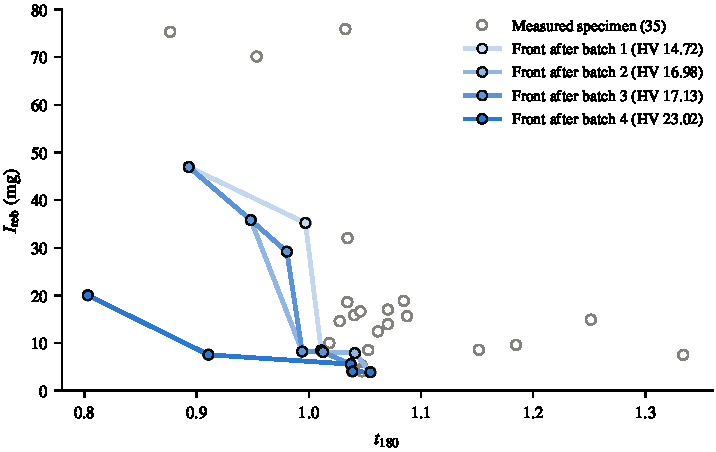
\includegraphics[width=0.8\textwidth]{figures/bo/t3-prism-bo-front-evolution.pdf}
  \caption{Measured objective space and front evolution across the
    four batches. The vertical axis is the mass-weighted rebound index
    $I_{\mathrm{reb}} = m\,e_{\mathrm{reb}}^{2}$ of
    Eq.~\eqref{eq:objectives}. Gray circles are
    the 35 first-print specimens with both objectives, at their
    stabilized means. The blue lines
    are the non-dominated fronts after each batch, with the dominated
    hypervolume (HV) at the $(1.35, \SI{50}{mg})$ reference in the
    legend. Batch 2 grew the front on the $I_{\mathrm{reb}}$ axis,
    batch 3 filled the knee, and batch 4 extended it to lower
    transmissibility. We draw repeated batch-3 designs at their
    first-print values.
    Lower is better on both axes.}
  \label{fig:front-evolution}
\end{figure*}

\subsection{Seed-Batch Measurements}
\label{sec:results:seed}

We printed all nine Sobol designs and the reference prism. Nine
specimens completed seed sessions: seven mapped Sobol designs, the
reference prism, and one specimen (amdjwm) whose design mapping is
unconfirmed. Specs 03 and 06 were printed, but their sessions are
absent from the campaign record, so they enter no fit or figure (the
nine seed geometries are drawn in Fig.~S3).
Table~\ref{tab:seed-results} reports the stabilized objectives. The
measured $t_{180}$ spans 0.893 to 1.062, and six of nine specimens
\emph{amplify} the peak shock reaching the top vertex. The print of
Sobol spec~01 (6lhxfy), the thick-strut, thin-cable, high-twist corner
of the batch, attenuated ($t_{180} = 0.893$), and a shorter, separate
seating of the same specimen on the previous day read within 0.14\% of
that value (33 stabilized drops, with a slight downward drift). The
spread between
specimens far exceeds the 0.17 to 0.48\% within-session per-drop CV,
but one specimen per geometry cannot separate geometry effects from
print-to-print variation. The best attenuator also had the largest
$I_{\mathrm{reb}}$ (\SI{46.9}{mg}), so the seed front is nondegenerate,
although the apparent trade-off rests largely on that one specimen
(Spearman $\rho = -0.39$, $p = 0.38$ over the seven mapped Sobol
designs). Printed mass and $t_{180}$ were strongly correlated over the
eight mapped specimens with weighed masses ($r = 0.82$), but the
correlation depends on the lightest specimen ($r = 0.26$ without
6lhxfy) and is confounded with geometry, so it is not evidence of a
mass effect. It motivated the constant-printed-mass batches that
followed (Section~\ref{sec:results:audits}).

\begin{table}[!tbp]
  \centering
  \caption{Seed-batch drop-tower results: 99 stabilized drops per
    specimen (101 for autv5r) after the 2 warm-up drops, at \SI{1.524}{m} (\SI{60}{in})
    onto the polyurethane surface, CFC-180 filtering. Means $\pm$ one
    standard deviation over the stabilized drops, ordered by $t_{180}$.
    $I_{\mathrm{reb}}$ uses each specimen's weighed mass
    (Eq.~\eqref{eq:objectives}). A dash marks a quantity the record
    cannot provide. Specimen \textit{amdjwm} lacks a weighed mass and a
    confirmed design mapping, so it is excluded from the surrogate fit
    and from every mass-dependent quantity. Specs 03 and 06 were printed
    but have no drop sessions in the campaign record.}
  \label{tab:seed-results}
  \small
  \begin{tabular}{@{}llS[table-format=2.2]S[table-format=1.4]@{\,$\pm$\,}S[table-format=1.4]S[table-format=2.1]@{}}
    \toprule
    Design & Specimen & {Mass (g)} & \multicolumn{2}{c}{$t_{180}$} &
    {$I_{\mathrm{reb}}$ (mg)} \\
    \midrule
    Spec 01 & 6lhxfy & 18.50 & 0.8931 & 0.0042 & 46.9 \\
    (unmapped) & amdjwm & {-} & 0.9805 & 0.0025 & {-} \\
    Spec 05 & 6nheas & 21.73 & 0.9970 & 0.0032 & 35.2 \\
    S0 ref. & bpx68c & 20.23 & 1.0111 & 0.0024 & 8.5 \\
    Spec 07 & ajhby6 & 20.53 & 1.0127 & 0.0038 & 8.1 \\
    Spec 00 & 9hhbkp & 21.62 & 1.0183 & 0.0017 & 10.0 \\
    Spec 04 & nvxsrv & 20.66 & 1.0275 & 0.0044 & 14.6 \\
    Spec 02 & autv5r & 22.04 & 1.0404 & 0.0035 & 15.8 \\
    Spec 08 & bag26v & 21.42 & 1.0616 & 0.0051 & 12.4 \\
    \bottomrule
  \end{tabular}
\end{table}

\subsection{Model-Recommended Batches and Replication}
\label{sec:results:batches}

Table~\ref{tab:batch-results} reports the stabilized objectives of the
three model-recommended batches. We evaluate Pareto membership over the
35 specimens with both objectives (amdjwm has no weighed mass).
Dominated hypervolume at the fixed reference
$(t_{180}, I_{\mathrm{reb}}) = (1.35, \SI{50}{mg})$, just beyond the
worst specimen on each axis through batch 2, grew from 14.72 after the
seed batch to 16.98 after batch 2 ($+15.3\%$), 17.13 after batch 3
($+0.9\%$), and 23.02 after batch 4 ($+34.4\%$), a 56\% total gain (65\%
for $E_{\mathrm{reb}}$ at its analogous reference, $(1.35, \SI{15}{mJ})$).
Two qualifications bound what this shows. First, hypervolume can only
grow as specimens are added, and we ran no budget-matched physical
baseline, so the comparison the data support is against the campaign's
own Sobol seed. The simulated campaign (Section~\ref{sec:results:sim})
supplies a budget-matched comparison, in simulation. Second, the batch-4 gain rests on two
single-seating specimens. Without corny7, whose re-seat is pending, the
total gain is 35\% (hypervolume 19.85), and without corny7 and corny6
batch~4 adds nothing. After batch 4 every member of the front (corny7,
corny6, drran5, drran3, r2d2c6) came from a model-recommended batch, and
corny7 and corny6 displaced the last seed members, 6lhxfy and ajhby6.
Because 27 of the 35 specimens came from those batches, though, a
five-member front drawn at random from them would be all
model-recommended about a quarter of the time. Scoring each batch-3
design at the mean of its screened prints
(Table~S6) removes drran5 and drran3
from the final front, leaves corny7, corny6, corny4, and r2d2c6, and
reduces batch 3's hypervolume gain from 0.9 to 0.1\%, so most of that
gain came from favorable first prints.

\paragraph{Batches 2 to 4} Batch 2 (trials 10 to 18) was printed under
the constant-solid-mass projection, so its masses spread from 17.91 to
\SI{23.47}{g}. It grew the front almost entirely on the
$I_{\mathrm{reb}}$ axis, and r2d2c6 still holds the lowest
$I_{\mathrm{reb}}$ on record (\SI{3.9}{mg}), a value bounded by the
second-contact search window (Section~\ref{sec:methods:testing}). Its archived
transmissibility predictions were optimistic for all nine specimens
(mean absolute percentage error, MAPE, 14.4\%, against 8.6\% for simply
predicting the mean of the training data), worst for r2d2c3 (predicted
0.910, measured 1.334, the strongest amplifier in the campaign). Batch 3
(trials 28 to 36), the first at constant printed mass (19.24 to
\SI{20.06}{g}) and the first with the infill and filament axes active,
filled the knee of the front. Its MAPE of 3.8\% matched the training
mean's 3.7\%, and its two first-print extremes did not hold up on later
prints: the best-predicted design (trial 32, predicted 1.020) measured
1.251, and the drift-flagged drran8 (trial 35) measured 0.980. Batch 4
(trials 37 to 45) split between the wide, high-twist, thin-cable family
the acquisition had favored since batch 2 and a previously unvisited
tall, low-twist corner. Four of its nine specimens attenuate, all from
the wide family. Specimen corny7, the batch's best-predicted design
(trial 37, predicted $0.934 \pm 0.13$), measured
$t_{180} = 0.8031 \pm 0.0025$, 10\% below the best seed specimen and
21\% below the reference prism, with $I_{\mathrm{reb}} = \SI{20.0}{mg}$,
so it dominates the seed attenuator on both objectives
(Fig.~\ref{fig:batch4-pred-vs-meas}). The archived predictions ranked
the nine specimens with Spearman $\rho = 0.82$ and the four attenuators
in the measured order, although the five amplifier predictions span only
0.9\%, and the batch MAPE was 6.0\%, against 9.6\% for the training mean. All four attenuators pass the seat
gauge (0.98 to 1.06), but under the between-seat rule their values,
the record included, are single-seating measurements whose re-seats
are pending. One session (corny5) carries a drift flag, and corny6 was
erratic (per-drop CV 2.0\%) but attenuates under any reading of its
record. We defined the seat gauge after batch 3, and only the three
prints of that batch were screened with it. Applied retrospectively, it
flags 10 of the 35 first-print sessions (two seed, five of batch 2, one
of batch 3, and two of batch 4), among them r2d2c3 (gauge 1.86), the
highest transmissibility in the campaign. None of these was re-seated,
and Tables~\ref{tab:seed-results} and~\ref{tab:batch-results} report
them unscreened.

\paragraph{Replication: three prints of batch 3} We printed the batch-3
plate three times and drop-tested every specimen under the same protocol,
540 drops in all (Fig.~\ref{fig:three-print}; per-print values in
Table~S6). Specimens 2dran$N$ and
dran3$N$ re-print drran$N$ at the same Ax trial. Neither first-print
extreme recurred. Trial 32 (drran7, 1.2513) measured 1.0286 and 1.0448
on its later prints, close to its prediction of 1.020, and the
attenuator of trial 35 (drran8, 0.9804) measured 1.0109 and 0.9958.
Trial 35 is the lowest-transmissibility design in every print, but its
screened mean is 1.003, so batch 3 contains no reproducibly attenuating
design. Every large same-design deviation came with a failed seat gauge.
The four sessions at or above the gauge threshold were each their design's highest
value, 4.5 to 19.8\% above the design's median, while the 23 below the
threshold sat a median 0.2\% from it (gauge versus deviation, Spearman
$\rho = 0.52$, $p = 0.006$). The third print supplied one new outlier,
dran35 (trial 28), at 1.168 with a gauge of 2.43 against 1.037 and 1.060
for its earlier prints, and its re-seat is pending.

Setting aside the four gauge failures and the two drift-flagged
sessions leaves 21 of the 27. One mean per design plus one offset per
print fits them with a residual standard deviation of 0.0087 in
$t_{180}$ (10 degrees of freedom), an order of magnitude above the
within-session standard errors the surrogate ingests (median 0.0006).
Over the screened sessions the intraclass correlation of $t_{180}$, the
share of its variance that lies between designs, is 0.58, against 0.06
with every session included. Most of that design signal comes from trial
35. The other eight design means, adjusted for the print offsets, span
only 1.028 to 1.045, less than the scatter of a single specimen, and the
orderings from different prints
agree poorly (Spearman $\rho$ of 0.08, 0.67, and 0.20 between pairs of
prints). The frozen batch-3 predictions rank the nine design means with
$\rho = 0.75$ ($p = 0.02$) after adjusting each mean for the print
offsets and $\rho = 0.55$ ($p = 0.12$) without that adjustment.
$I_{\mathrm{reb}}$ repeats far less well. For each design the largest of
its three values is 1.9 to 8.3 times the smallest, the rank correlations
between prints are $-0.18$, 0.25, and 0.33, and the scatter between
prints (standard deviation \SI{17.0}{mg}) exceeds the spread of the
design means (\SI{10.2}{mg}). The 1.2513 session had passed every
within-session stability check (per-drop CV 0.77\%, no drift), which is
why we adopted the between-seat replication rule. The nine second-print
specimens joined the surrogate's training set, while the third print
(sessions of 2026-09-28 to 2026-10-02) postdates the most recent refit
and enters neither the fits, the cross-validation, nor
Fig.~\ref{fig:front-evolution}.

\begin{table*}[!tbp]
  \centering
  \caption{Model-recommended batch results, one row per Ax trial in
    ascending order, under the protocol and reporting conventions of
    Table~\ref{tab:seed-results} (CFC-180, stabilized means $\pm$ one
    standard deviation). The italic line above each batch gives its
    mass basis and the filament settings of its print job, read from the
    archived slicer project for batch 2 and from the design record for
    batches 3 and 4. Columns $R$ to $d_t$ and the two infill densities
    are the commanded values after the constant-mass projection, and
    batch 2 did not vary infill. Each specimen received 18 to 20
    stabilized drops against the seed batch's 99, and the archived per-drop
    records give the exact per-session counts. $m$ is the weighed
    specimen mass, and $I_{\mathrm{reb}}$, the mass-weighted rebound index of
    Eq.~\eqref{eq:objectives} (lower is better), uses it. ``Pred.''\ is
    the posterior-mean $t_{180}$ archived when the model recommended the batch,
    before we tested any of its specimens. $\dagger$ marks a
    transmissibility-drift-flagged session whose mean is provisional,
    and $\ddagger$ marks an erratic session (per-drop CV above 1.5\%
    without a drift flag). The print key
    (Table~S4 of the Supplementary Information)
    maps each trial to its specimen.}%
  \label{tab:batch-results}
\footnotesize
\setlength{\tabcolsep}{7.5pt}
\begin{tabular}{@{}lS[table-format=2.1]S[table-format=3.1]S[table-format=2.1]S[table-format=2.2]S[table-format=1.2]S[table-format=2.0]S[table-format=2.0]S[table-format=2.2]S[table-format=1.4]@{\,$\pm$\,}S[table-format=1.4]S[table-format=2.1]S[table-format=1.3]@{}}
  \toprule
  Trial & {$R$} & {$H$} & {$\theta$} & {$d_s$} & {$d_t$} &
  \multicolumn{2}{c}{Infill (\%)} & {$m$} & \multicolumn{2}{c}{$t_{180}$} &
  {$I_{\mathrm{reb}}$} & {Pred.} \\
  \cmidrule(lr){7-8}
  & {(mm)} & {(mm)} & {(deg)} & {(mm)} & {(mm)} & {PLA} & {TPU} & {(g)} &
  \multicolumn{2}{c}{mean $\pm$ sd} & {(mg)} & {$t_{180}$} \\
  \midrule
    \multicolumn{13}{@{}l}{\textit{Batch 2, constant solid mass, infill not varied. PLA at 220\,\si{\celsius} and \SI{30}{mm^3/s}, TPU at 240\,\si{\celsius} and \SI{2.5}{mm^3/s}.}} \\
    10 & 21.9 & 52.7 & 80.0 & 10.53 & 2.63 & {-} & {-} & 17.91 & 1.0530 & 0.0035 & 8.5 & 0.873 \\
    11 & 30.1 & 45.2 & 80.0 & 9.04 & 4.14 & {-} & {-} & 19.33 & 1.1847 & 0.0076 & 9.6 & 0.885 \\
    12$^\dagger$ & 22.5 & 53.9 & 40.0 & 10.78 & 2.70 & {-} & {-} & 17.96 & 1.0411 & 0.0154 & 7.9 & 0.926 \\
    13 & 27.3 & 65.5 & 80.0 & 8.08 & 3.28 & {-} & {-} & 19.38 & 0.9942 & 0.0021 & 8.2 & 0.948 \\
    14 & 20.4 & 49.0 & 40.0 & 9.79 & 4.49 & {-} & {-} & 19.11 & 1.0548 & 0.0042 & 3.9 & 0.953 \\
    15 & 34.9 & 52.3 & 40.0 & 10.47 & 2.62 & {-} & {-} & 18.51 & 0.9484 & 0.0008 & 35.8 & 0.905 \\
    16 & 20.1 & 48.2 & 80.0 & 9.63 & 4.42 & {-} & {-} & 18.63 & 1.3337 & 0.0117 & 7.5 & 0.910 \\
    17 & 26.9 & 74.0 & 80.0 & 8.08 & 3.70 & {-} & {-} & 19.98 & 1.0704 & 0.0116 & 14.0 & 0.955 \\
    18 & 25.1 & 60.1 & 80.0 & 6.01 & 5.51 & {-} & {-} & 23.47 & 1.1516 & 0.0040 & 8.6 & 0.987 \\
  \midrule
    \multicolumn{13}{@{}l}{\textit{Batch 3, constant printed mass (20.23 g). PLA at 217\,\si{\celsius} and \SI{20.5}{mm^3/s}, TPU at 244\,\si{\celsius} and \SI{3.6}{mm^3/s}.}} \\
    28 & 23.2 & 55.8 & 40.0 & 5.58 & 5.11 & 21 & 29 & 19.88 & 1.0373 & 0.0024 & 5.6 & 1.059 \\
    29 & 27.8 & 76.5 & 40.0 & 8.35 & 3.83 & 13 & 31 & 19.92 & 1.0344 & 0.0017 & 18.6 & 1.032 \\
    30 & 23.0 & 55.2 & 40.0 & 5.52 & 5.06 & 31 & 18 & 19.34 & 1.0425 & 0.0009 & 6.3 & 1.058 \\
    31 & 20.7 & 65.1 & 40.0 & 9.04 & 4.14 & 18 & 21 & 19.92 & 1.0389 & 0.0012 & 4.0 & 1.043 \\
    32 & 29.9 & 60.6 & 40.0 & 8.10 & 4.11 & 24 & 13 & 20.06 & 1.2513 & 0.0096 & 14.9 & 1.020 \\
    33 & 23.1 & 55.4 & 40.0 & 5.54 & 5.08 & 29 & 16 & 19.33 & 1.0345 & 0.0006 & 32.0 & 1.056 \\
    34 & 21.7 & 52.1 & 40.0 & 8.81 & 4.78 & 16 & 34 & 19.24 & 1.0471 & 0.0040 & 5.3 & 1.065 \\
    35$^\dagger$ & 25.3 & 60.8 & 61.5 & 9.02 & 3.04 & 26 & 24 & 19.32 & 0.9804 & 0.0051 & 29.2 & 1.039 \\
    36 & 25.9 & 62.1 & 40.0 & 8.27 & 3.11 & 34 & 26 & 19.31 & 1.0326 & 0.0016 & 75.9 & 1.051 \\
  \midrule
    \multicolumn{13}{@{}l}{\textit{Batch 4, constant printed mass (20.23 g). PLA at 226\,\si{\celsius} and \SI{29.5}{mm^3/s}, TPU at 236\,\si{\celsius} and \SI{2.6}{mm^3/s}.}} \\
    37 & 34.3 & 67.1 & 79.0 & 8.98 & 2.58 & 22 & 21 & 19.62 & 0.8031 & 0.0025 & 20.0 & 0.934 \\
    38 & 18.3 & 80.3 & 40.0 & 7.98 & 4.02 & 18 & 34 & 20.21 & 1.0846 & 0.0030 & 18.8 & 1.008 \\
    39 & 34.7 & 68.3 & 80.0 & 8.86 & 2.60 & 21 & 34 & 19.64 & 0.9535 & 0.0025 & 70.1 & 0.954 \\
    40$^\dagger$ & 20.8 & 91.6 & 40.0 & 5.00 & 4.58 & 18 & 21 & 20.58 & 1.0876 & 0.0099 & 15.6 & 1.012 \\
    41$^\ddagger$ & 33.4 & 67.3 & 80.0 & 8.65 & 2.51 & 29 & 18 & 19.45 & 0.9106 & 0.0181 & 7.5 & 0.943 \\
    42 & 17.7 & 77.7 & 40.0 & 8.47 & 3.88 & 19 & 34 & 20.20 & 1.0459 & 0.0029 & 16.6 & 1.010 \\
    43 & 37.1 & 65.5 & 80.0 & 9.25 & 2.78 & 12 & 29 & 19.46 & 0.8766 & 0.0036 & 75.3 & 0.942 \\
    44 & 20.8 & 91.5 & 40.0 & 4.99 & 4.58 & 19 & 21 & 20.56 & 1.0475 & 0.0025 & 4.1 & 1.013 \\
    45 & 19.7 & 86.5 & 40.0 & 6.89 & 4.32 & 12 & 35 & 20.15 & 1.0705 & 0.0013 & 17.0 & 1.004 \\
  \bottomrule
\end{tabular}
\end{table*}

\begin{figure*}[!tbp]
  \centering
  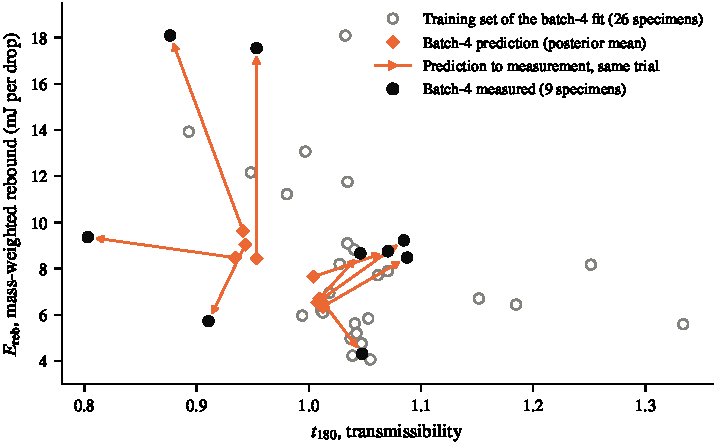
\includegraphics[width=0.8\textwidth]{figures/bo/t3-prism-bo-round4-predicted-vs-actual.pdf}
  \caption{Batch-4 predictions against outcomes. Orange diamonds are the
    archived posterior-mean predictions for trials 37 to 45, saved when
    the optimizer recommended the batch, and each arrow joins a prediction to the
    measured value of the specimen printed for the same trial (black).
    Gray circles are the 26 specimens we trained the batch-4 fit on
    (the seed batch, batch 2, and the first prints of batch 3). The
    vertical axis is $E_{\mathrm{reb}}$, the first-power form of
    Section~\ref{sec:methods:testing} that the optimizer predicted and
    minimized when it recommended the batch.
    Figure~\ref{fig:front-evolution} plots $I_{\mathrm{reb}}$ instead. We omit predictive uncertainty
    for legibility. The record attenuator corny7 (measured 0.803) is the
    left-most point. Lower is better on both axes.}
  \label{fig:batch4-pred-vs-meas}
\end{figure*}

\begin{figure*}[!tbp]
  \centering
  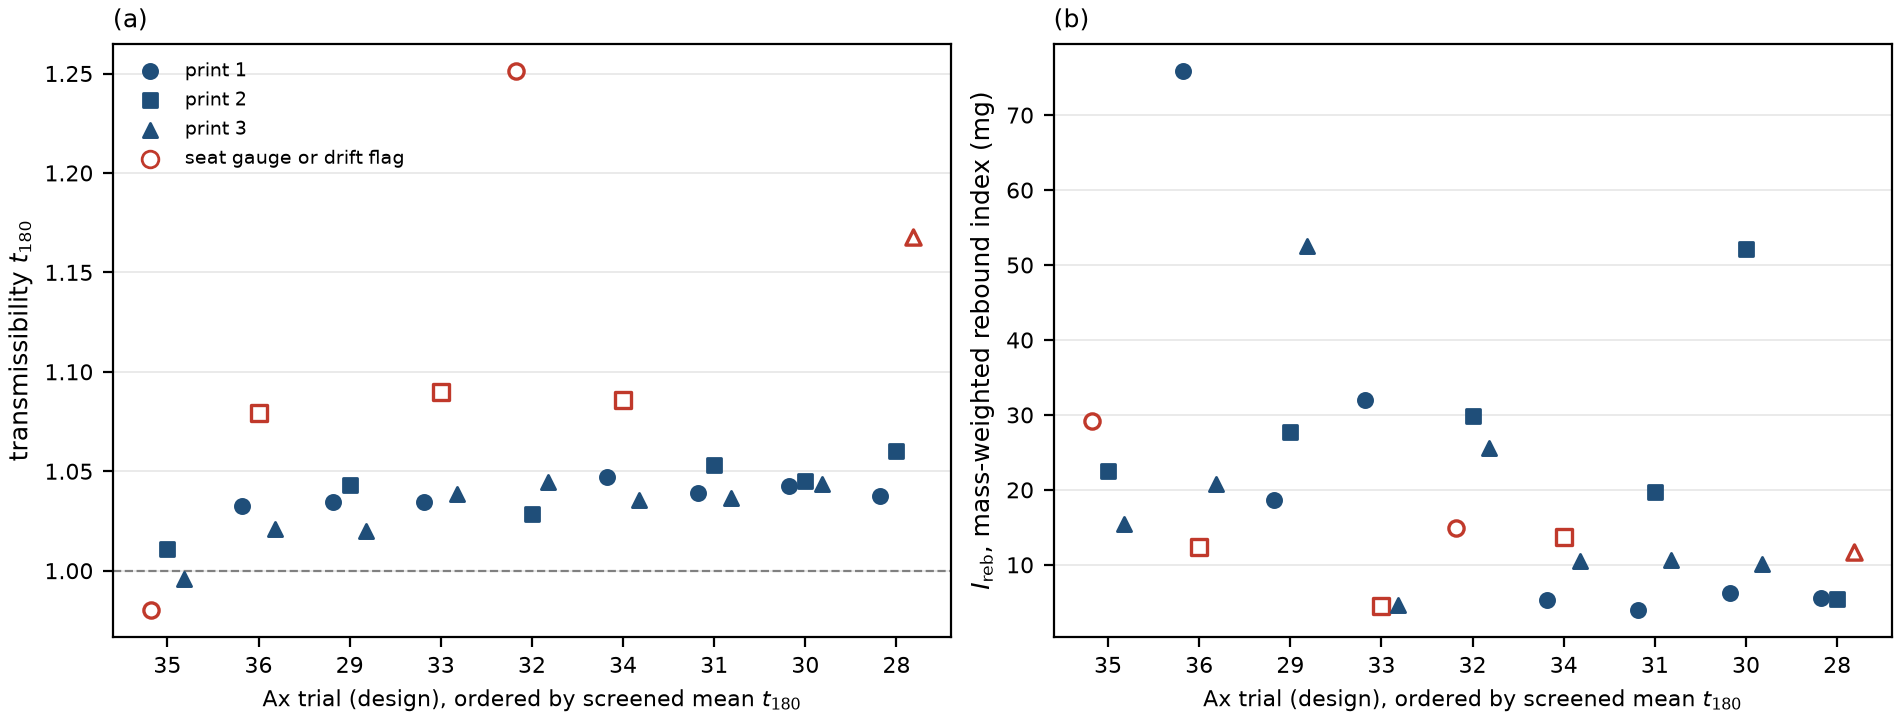
\includegraphics[width=\textwidth]{figures/analysis/round3-three-print.png}
  \caption{Three prints of each batch-3 design. \emph{(a)} Transmissibility
    and \emph{(b)} $I_{\mathrm{reb}}$ for print 1 (circles), print 2
    (squares), and print 3 (triangles), with the designs ordered by their
    screened mean transmissibility. Open red markers are sessions with a
    failed seat gauge or a drift flag, which the screened means leave out.
    The dashed line marks $t_{180} = 1$.}
  \label{fig:three-print}
\end{figure*}

\subsection{Surrogate Audits Across the Campaign}
\label{sec:results:audits}

We audited each refit by cross-validation, with one full NUTS refit per
held-out fold. Held-out point accuracy declined as the campaign grew:
the leave-one-out $t_{180}$ MAPE rose from 2.9\% on the seed state to
6.2\% after batch 3, while the input space doubled from 6 to 12 and
batch 3 added the campaign's largest outliers
(Section~S14). Once replicates exist, leave-one-out
leaks, because a held-out print's twin stays in training at nearly the
same coordinates. We therefore re-audited the fit's 44-specimen
training record with leave-one-design-out folds (35 folds, each
drran/2dran pair held out together, at the full NUTS budget). The
$t_{180}$ MAPE is 4.8\% with Spearman $\rho_s = +0.32$ (two-sided
permutation $p = 0.036$), but the held-out predictions stay near the
pooled mean, with about a third of the measured spread
(Fig.~S6). For $E_{\mathrm{reb}}$ the MAPE is 38.8\%
and $\rho_s = -0.40$ ($p = 0.008$). These rank correlations need a
reference: a predictor that returns each fold's training mean scores
$\rho_s = -0.87$ for $t_{180}$ and $-0.79$ for $E_{\mathrm{reb}}$ on the
same folds by construction, because holding out a high value raises the
mean of the rest. The negative $E_{\mathrm{reb}}$ value therefore
reflects predictions that barely depart from the pooled mean, not an
inverted ordering, and the out-of-sample coefficient of determination
against each fold's training mean, which is zero for that predictor, is
the cleaner summary: 0.12 for $t_{180}$ and $-0.05$ for
$E_{\mathrm{reb}}$. An earlier run of the same folds at a quarter of the
NUTS budget gave $\rho_s = +0.08$ for $t_{180}$, so the ranking statistic
also depends on how fully each fold's posterior is sampled. The campaign
surrogate therefore had little held-out skill on $t_{180}$ and none on
rebound. Its value to the campaign lay in
the region it steered batch 4 toward, where its prospective ranking held
up (Section~\ref{sec:results:batches}), rather than in point forecasts.

\paragraph{Noise specification} The weak held-out skill comes mostly
from the noise model rather than from a lack of signal. The campaign
fits take each specimen's within-session standard error as a known noise
variance, while prints of one design differ by an order of magnitude
more. To explain those differences the fit leans on the one input that
differs between reprint twins, their weighed mass. Fitted to all 44
specimens, it gives printed mass the largest share of the model
sensitivity, at a length scale of 0.04 of the unit cube for $t_{180}$
and 0.013 for $E_{\mathrm{reb}}$, and its posterior mean is nearly flat
away from the data (Fig.~S5). Refitting the same
model on the same folds with one noise variance per objective learned
from the data, and nothing else changed, raised the held-out $\rho_s$
to $+0.55$ for $t_{180}$ and $+0.51$ for $E_{\mathrm{reb}}$ (both
$p < 0.001$), and the out-of-sample coefficient of determination against
the mean of each training fold from 0.12 to 0.40 and from $-0.05$ to
0.23. In the learned-noise fit, cable diameter $d_t$ carries the largest
share of the $t_{180}$ sensitivity in all four NUTS chains, followed by
the twist angle. A tuned random forest on the same folds ranks held-out
$t_{180}$ about as well ($\rho_s = +0.52$) and $E_{\mathrm{reb}}$ less
well ($+0.27$, $p = 0.08$), and point-estimated GPs with learned noise
rank about as well as SAASBO ($\rho_s$ of 0.48 to 0.55 for $t_{180}$ and
0.41 to 0.54 for $E_{\mathrm{reb}}$), so we make no claim that SAASBO
ranks better. Its posterior standard deviation is better calibrated for
$t_{180}$, covering 41 of the 44 held-out values (93\%) at 1.96
standard deviations against 77 to 89\% for the point-estimated GPs. Its
$E_{\mathrm{reb}}$ intervals, which leave out the learned noise, cover
only 73\%. This is a
post hoc re-analysis of the same 44 specimens. The fixed-noise model
chose batches 2 to 4, and its archived predictions are the ones
Table~\ref{tab:batch-results} reports.

\paragraph{Mass} The correlation between printed mass and
transmissibility fell from $r = 0.82$ over the eight mapped seed
specimens to $0.12$ over all 53 specimens with a weighed mass ($r^2 = 0.01$), so the
seed correlation did not persist once printed mass was held near
constant. Within batch 4 the two correlate strongly
($r = 0.85$), but there the wide, high-twist family printed at 19.45 to
\SI{19.64}{g} and the tall, low-twist family at 20.15 to
\SI{20.58}{g}, so printed mass follows the design family.

\subsection{Simulated Campaign}
\label{sec:results:sim}

Table~\ref{tab:sim-campaign} scores each run of the simulation-only
campaign (Section~\ref{sec:methods:sim}) by its final hypervolume as a
percentage of a best-known reference. That reference is the
hypervolume of a 16,384-design reference sweep, a locally refined
front, and every feasible design that any compared run evaluated. After 45 simulated
designs, BO reached 93.0\% of this reference (seed range 90.0 to
96.1\%), against 76.5 to 79.1\% for the four baselines. BO finished
ahead of every baseline on all ten seeds, and no baseline seed reached
the worst BO seed, so the one-sided exact Mann-Whitney $p$ is
$5.4\times10^{-6}$, the smallest value ten runs against ten allow. The
running hypervolume (Fig.~S7 of the
Supplementary Information) shows BO trailing the baselines during its
Sobol batch and pulling ahead once the model chooses the designs.

We chose this objective pair before running the campaign, by screening
six candidate pairs for the one whose front a random 45-design batch
covers least (Section~S15). The result therefore
shows that the optimizer finds a front that sampling misses when one
exists, not that it will on every pair. The control pair, $t_{180}$
with peak tendon strain, shows the other case. There a random batch
already collects about 85\% of the screening sweep's hypervolume.
Against the best-known reference, BO reached 82.6\% and the baselines
77.4 to 79.8\%, and no comparison survives a four-way
Bonferroni correction (smallest one-sided exact Mann-Whitney $p = 0.018$). The control's
baselines also used an earlier protocol that charged unprintable
draws, so the two pairs are not a controlled contrast. Because the
simulated struts are rigid, the simulator keeps $t_{180}$ below about 1
and does not reproduce the amplification measured on hardware
(Section~\ref{sec:discussion}). The simulated campaign therefore tests
the optimizer only.

\begin{table}[!tbp]
  \centering
  \caption{Simulation-only campaign: final hypervolume after 45
    designs as a percentage of each objective pair's best-known
    reference (mean $\pm$ sample standard deviation over ten seeds).
    $p$ is the $p$-value of the one-sided exact Mann-Whitney test that BO exceeds the
    baseline, and Wins counts the seeds on which BO finished ahead of
    the baseline run with the same seed index. LHS is Latin hypercube
    sampling. The envelope-pair baselines skip unprintable candidates
    without simulating them, and the strain control used the earlier
    protocol that charged them.}%
  \label{tab:sim-campaign}
  \footnotesize
  \setlength{\tabcolsep}{3.5pt}
\begin{tabular}{@{}lccccc@{}}
  \toprule
  & \multicolumn{3}{c}{$t_{180}$ + envelope} & \multicolumn{2}{c}{$t_{180}$ + strain} \\
  \cmidrule(lr){2-4}\cmidrule(l){5-6}
  Method & HV (\%) & $p$ & Wins & HV (\%) & $p$ \\
  \midrule
  BO (qNEHVI) & 93.0 $\pm$ 2.2 &  &  & 82.6 $\pm$ 4.3 &  \\
  Random & 79.1 $\pm$ 2.7 & $5.4\times10^{-6}$ & 10/10 & 79.6 $\pm$ 4.2 & 0.14 \\
  Sobol & 77.3 $\pm$ 4.2 & $5.4\times10^{-6}$ & 10/10 & 79.8 $\pm$ 2.2 & 0.038 \\
  LHS & 76.5 $\pm$ 3.4 & $5.4\times10^{-6}$ & 10/10 & 78.8 $\pm$ 2.8 & 0.018 \\
  Compass & 78.1 $\pm$ 5.3 & $5.4\times10^{-6}$ & 10/10 & 77.4 $\pm$ 7.9 & 0.062 \\
  \bottomrule
\end{tabular}
\end{table}

\section{Discussion}
\label{sec:discussion}

\subsection{What the Campaign Establishes}
The loop closed three times on physical hardware, with each refit's
recommendations printed, measured, and fed back. The measurement
separates the tested specimens, whose $t_{180}$ means span 0.803 to
1.334, far beyond the within-session scatter, and the three prints of
batch 3 put the resolution floor for a single specimen at a standard
deviation of about 0.009 between clean seatings of different prints. The
physics is less favorable than the cushioning intuition suggests. At this
scale and rate most printed prisms \emph{amplify} the peak shock reaching
their top vertex (26 of the 36 first-print specimens), so the useful question became
which corner of the design space crosses into attenuation, and at what
cost in rebound. Batch 4 answered it with four attenuators from the wide,
high-twist, thin-cable family, led by its best-predicted design at
$t_{180} = 0.803$. The attenuators tend to rebound more. Specimens corny8 and
corny9 have the lowest velocity loss indices of the batch (0.940 and
0.938), and in the video check the share of arrival speed returned rises
as $t_{180}$ falls (Spearman $\rho = -0.59$ over 27 specimens;
Section~S8), so the front stays two-dimensional.

\subsection{Pre-Registered Review of the Objective Choices}
\label{sec:discussion:review}
We
pre-registered an adversarial, data-first review of the objective choices
and ran it with the analysis tool named in Section~\ref{sec:methods:ai}; the
review had to commit to its own objective set from the raw campaign files
before reading ours. It found that the rebound fraction rests on an
unvalidated ballistic reading of the second contact, that the apparent
seed-batch trade-off depends on the single strongest attenuator
(Spearman $\rho = -0.39$, $p = 0.38$), and that per-drop standard errors
understate design-level uncertainty. The campaign responded to all
three. The three prints of batch 3 measured the understatement directly,
at an order of magnitude in $t_{180}$, and a re-analysis that learns the
noise instead of supplying it ranks held-out designs above chance on both
objectives (Section~\ref{sec:results:audits}). The video check
(Section~\ref{sec:methods:testing}) showed that the ballistic reading
does not give the hop speed but ranks specimens similarly to the
measured rebound, so $e_{\mathrm{reb}}$ stays a ranking index and a
candidate constraint rather than a physical quantity. The between-seat
replication rule now gates every extreme, and the constant-printed-mass
projection holds batch masses within about 3\% of target, which narrows
the seed batch's mass confound (Section~\ref{sec:results:seed}). We
report this trajectory because the loop is the contribution, and its
second objective was revised after the final batch, in response to
these findings.

\subsection{Relation to Prior Art, and the Role of Simulation}
Relative
to Pajunen et~al.~\cite{pajunen2019design}, we vary the geometry under an
optimization loop rather than characterizing a single fabrication
condition. Relative to Mo et~al.~\cite{mo2023accelerated} and Hertlein
et~al.~\cite{hertlein2024latticeimpact}, whose objectives come from
computational models, the loop's ground truth is physical measurement,
and no simulated number enters the objectives, the acquisition, or
candidate priority. An exploratory
multi-engine simulation study, from rigid-body through finite-element
fidelity (archived in the repository; Data Availability Statement),
could not reproduce the amplification that dominates the measured
record. Its rigid-strut models cap $t_{180}$ near unity, and its rebound
predictions did not separate designs that the measurement separates.
Simulation shaped the campaign through the constant-mass fairness
constraint, and it supplies the budget-matched baseline comparison of
Section~\ref{sec:results:sim}, but it should show prospective predictive
skill on unseen specimens before it takes a larger role. The near-unity
transmission of most printed cells also cautions against reading the
printed-tensegrity literature's attenuation results as generic. The
present cells are not pretensioned, and activating genuine pretension in
printed tensegrity is an open direction outside this campaign.

\subsection{Path Forward}
No joint failed during the repeated-drop
sessions, which covered 1,614 stabilized captures across the 53 weighed
specimens, but those sessions were
not designed as fatigue tests, so interface durability remains open, and
pull-out and fatigue characterization of the internal-anchor joint is
planned. A replicate study re-printed three batch-4 designs (corny7,
corny8, and corny2) nine times each to test whether their ordering
survives print and seating variation. Its first plate was tested on
2026-10-17 with two instrument faults, testing stopped when the
base-input instrumentation failed on 2026-10-19, and we withhold that
partial record until the repeats are complete
(Section~S11). Also planned are the re-seat confirmations of the batch-4
attenuators, a metal-analog rank-transfer comparison
(Section~S12), quasi-static crush testing
(Section~S9), tiled multi-cell
absorbers~\citep{sabounizawadzka2024experimental}, and miniaturization
to walking-aid tips, where spring-loaded and polymer-damped tips reduce
loading rate but not peak transmitted
force~\citep{segura2007mechanicsofambulation,
macgillivray2016theinfluenceof} and tensegrity crutch concepts have been
proposed~\citep{gu2026tensegritycrutches}.

\subsection{Limitations}
The measured evidence base is 54 tested specimens: 36
across the four batches (35 with a weighed mass) and 18 re-prints of
the nine batch-3 designs, the only designs with more than one reported
test. Every single-specimen extreme, the batch-4 record included, is
provisional until its re-seat, and the batch-4 hypervolume gain depends
on two such specimens. Ten first-print sessions that the seat gauge
flags were never re-seated, and four rebound fractions, two of them on
the final front (drran3 and r2d2c6), are bounded by the second-contact
search window. Re-seating those specimens and re-processing with a
wider window would settle both. The surrogate
that chose the batches took the within-session standard errors as known
noise and had little held-out skill (out-of-sample coefficients of
determination of 0.12 for $t_{180}$ and $-0.05$ for $E_{\mathrm{reb}}$).
Learning the noise raises them to 0.40 and 0.23 in a re-analysis, but no
batch was chosen with that model. The drop protocol
probes one height, one impact surface, and axial loading only, and the
specimens stay elastic, so crush-energy metrics await the quasi-static
campaign, and the rig has no falling-mass or displacement channel from
which to integrate absorbed energy in joules. The rebound fraction is a
timing index, not a measured rebound velocity. The campaign's filters
pass about 20\% less bandwidth than SAE~J211/1 specifies
(Section~\ref{sec:methods:testing}), which leaves $t_{180}$ on the
illustrated drop unchanged but shifts the CFC-1000 seat gauge. The four
filament axes carry one value per batch and are not identifiable. One
tested seed specimen lacks a design mapping, one seed design's specimen
assignment (design 08) carries a recorded discrepancy
(Section~S6), and two seed designs have no
session record. All results come from one printer, material pair, and
cell topology.

\section{Conclusions}
\label{sec:conclusions}

We have presented an experiment-driven Bayesian-optimization framework
for the impact response of multi-material 3D-printed tensegrity-inspired
structures, in which TPU takes the place of the traditional tension
elements and PLA struts carry compression most of the time, and we have
run it through the recommend, fabricate, measure, and update cycle three
times on physical hardware. Across four measured
batches (36 specimens), transmissibility spanned 0.803 to 1.334, and most
specimens amplified the peak shock. The dominated hypervolume grew 56\%
over the Sobol seed front, every member of the final front came from a
model-recommended batch, and the final batch's best-predicted design
reached $t_{180} = 0.803$, 10\% below the best seed specimen, a value
that awaits its re-seat confirmation. For design, the record points to
wide, high-twist prisms with thin cables as the corner where these cells
attenuate, at the cost of more rebound, with cable diameter and twist
leading the $t_{180}$ sensitivity of the learned-noise surrogate. Printing one batch's nine designs
three times put the print-to-print standard deviation of the
transmissibility at 0.009, an order of magnitude above the standard
error of a session mean, and a broadband seat gauge flagged both of the
largest single-print errors, so a single-print extreme needs a
replicate, or at least a clean re-seat, before it counts. In a
simulation-only benchmark, BO collected 93\% of the best-known
hypervolume in 45 designs where three space-filling samplers and a compass search collected 76.5 to
79.1\%, but on a control objective pair that sampling alone covers well,
BO did not separate from the samplers. The workflow suits other
experimentally evaluated architected structures whose constitutive
response is hard to calibrate from first principles, although transfer
beyond this printer, material pair, topology, and axial impact condition
remains untested.

\section*{Acknowledgments}

The Brigham Young University Mentored Research Grant program supported
this work. The authors thank the undergraduate researchers
who carried out the multi-material printing and impact testing, and the
graduate co-mentor who supported day-to-day operations.

\section*{AI Use Statement}

We used AI tools under our direction throughout this project, for code,
analysis, figures, and manuscript text, and we reviewed their output at
every step. Claude Code (Anthropic) ran mostly as a GitHub Action, from
June to November 2026, and in local command-line sessions from September
to October 2026, with the models Claude Opus 4.8, Opus 5, Opus 5.5,
Fable 5, and Fable 5.1. The GitHub Copilot coding agent, mostly with
Claude Opus 4.6 to 4.8, worked on the project from March to July 2026,
and the Copilot command-line interface and Copilot Autofix were used
between March and June 2026. The Edison Scientific platform produced mock
peer reviews of earlier drafts, literature and reference checks, the
review of the objective choices in Section~\ref{sec:discussion:review},
and an audit of the simulated campaign, from May to September 2026. The
faster-whisper speech-to-text model transcribed the co-authors' recorded
reviews of the draft. Section~\ref{sec:methods:ai} describes how we
checked this work, and the repository file \texttt{manuscript/AI-USE.md}
(Data Availability Statement) lists each tool, model, access route, and
date range, with every automated run on the manuscript. The human authors
have reviewed the manuscript in full and take responsibility for it.

\section*{Conflict of Interest}
The authors declare no conflict of interest.

\section*{Data Availability Statement}

The code and data behind this paper are public in the GitHub repository
\url{\repo}. The repository has no tagged release yet, so we cite each
part by the commit that holds it, and each commit can be browsed at
\texttt{\repo/tree/}\textit{commit}:
\begin{itemize}
  \item the data snapshot behind every table and figure, with the scripts
    that regenerate them, the cross-validation fold records, the surrogate
    re-analysis, and the inventory of AI-tool use
    (\texttt{manuscript/AI-USE.md}): commit
    \href{\repo/tree/7fce855563f6aa372911d6562cbebe8124553ea3}{\texttt{7fce855}}
    (pull request~76);
  \item the Bayesian-optimization campaign code, with the experiment
    state, recommendations, and archived predictions of each round, the
    slicer project of each printed batch, and the parametric CAD model of
    the $T_3$ prism: commit
    \href{\repo/tree/65ff9788a363025746463a463f10d3da7456ac11}{\texttt{65ff978}};
  \item the drop-test processing pipeline and the per-drop records of the
    campaign sessions: commit
    \href{\repo/tree/f6471adb34cb5f2d0eba571d5005f4e250241fec}{\texttt{f6471ad}};
  \item the exploratory simulation study and the simulation-only campaign:
    commit
    \href{\repo/tree/94e53a8efa331bb53855f971d998d95e5ef89b14}{\texttt{94e53a8}}
    (pull request~33);
  \item the video tracking behind the rebound check: commit
    \href{\repo/tree/4e4c0c2405dce793bcc53369c896ac078fa957f8}{\texttt{4e4c0c2}};
  \item the joint-design study: commit
    \href{\repo/tree/2a644f5844d9fe9460a2bcf641ca5e99e0fe3666}{\texttt{2a644f5}}
    (pull request~39).
\end{itemize}
Three things are not yet public. The raw high-speed videos are not in the
repository, which holds the tracking results and annotated frames instead.
The repository has no license file yet, so the terms for reusing the code
and data are not stated. No versioned archive with a DOI exists yet.

\section*{Nomenclature}
\begingroup
\small
\begin{longtable}{@{}p{0.24\textwidth}p{0.72\textwidth}@{}}
  \multicolumn{2}{@{}l}{\textit{Latin symbols}}\\[2pt]
  $a_{\mathrm{base}}$ & base-plate acceleration, filtered (G, multiples of standard gravity)\\
  $\mathbf{a}_{\mathrm{top}}$ & top-vertex acceleration vector, filtered (G)\\
  $d_j$ & joint diameter (mm)\\
  $d_s$ & strut diameter (mm)\\
  $d_t$ & cable (tendon) diameter (mm)\\
  $E_{\mathrm{reb}}$ & first-power mass-weighted rebound,
    $e_{\mathrm{reb}}\,m\,g\,h$ (mJ)\\
  $e_{\mathrm{reb}}$ & rebound fraction, Eq.~\eqref{eq:objectives} (dimensionless)\\
  $g$ & gravitational acceleration (\si{m/s^2})\\
  $H$ & cell height between the joint-center planes (mm)\\
  $h$ & drop height (m)\\
  $I_{\mathrm{reb}}$ & mass-weighted rebound index,
    $m\,e_{\mathrm{reb}}^2$ (mg)\\
  $m$ & weighed specimen mass (g)\\
  $m^{\star}$ & solid CAD mass target of batches 1 and 2 (g)\\
  $N_x, N_y, N_z$ & number of cells along each axis of a tiling\\
  $n_{\mathrm{drops}}$ & stabilized drops in a session\\
  $q$ & batch size (specimens per batch)\\
  $R$ & circumradius of the end triangles (mm)\\
  $r$ & Pearson correlation coefficient\\
  $s_{\mathrm{drop}}$ & per-drop standard deviation within a session\\
  $t_{180}$ & transmissibility, CFC-180 peak acceleration ratio\\
  $t_{\mathrm{second}}$ & time from impact to the second contact (s)\\
  VLI & velocity loss index, $1 - e_{\mathrm{reb}}$\\[4pt]
  \multicolumn{2}{@{}l}{\textit{Greek symbols}}\\[2pt]
  $\Delta v$ & base velocity change through the impact (m/s)\\
  $\theta$ & twist angle between the end triangles (deg)\\
  $\rho$, $\rho_s$ & Spearman rank correlation coefficient\\
  $\sigma_e$, $\sigma_I$, $\sigma_m$, $\sigma_t$ & standard errors
    of $e_{\mathrm{reb}}$, $I_{\mathrm{reb}}$ and $t_{180}$, and the
    standard deviation of printed mass\\
\end{longtable}
\endgroup

\bibliographystyle{unsrtnat}
\bibliography{journal-strings,references}

\end{document}
